\documentclass[12pt]{article}

\usepackage[top=50pt, bottom=50pt, left=90pt, right=90pt]{geometry}
\usepackage[pdftex]{graphicx}
\usepackage{soul}

\usepackage{lipsum}%% a garbage package you don't need except to create examples.
\usepackage{fancyhdr}
\pagestyle{fancy}

%This is some header and footer information
\lfoot{Kids Coding Club}
\rfoot{\thepage}
\cfoot{}
\renewcommand{\headrulewidth}{0pt}
\renewcommand{\footrulewidth}{0.4pt}

%Basic title information about original author and title
\title{Class 5 - Analog Arduino}
\author{Chris Hight}
\date{\today}
 

\begin{document}

\maketitle


\section *{Introduction to the Project}
	\begin{itemize}
		\item During this project we are going to setup a temperature sensor to the arduino analog pins, when our reading reaches a certain level a LED turns on.

		\item The parts we are going to use are:
	
		\begin{itemize}
    		\item Arduino - This is our brain
    		\item Breadboard - This is how we can connect arduino and parts together
    		\item LED - This is a light
    		\item Resistor - This restricts how much electricity we let run through the circuit
    		\item Temperature Sensor - This converts temperature to voltage
		\end{itemize}
		
		\item In the second hour you may get to the line sensor programming, that will be very similar to the way the temperature sensor is setup
	
	\end{itemize}



\section *{Connecting the temperature sensor}
	\begin{itemize}
		\item We are going to start with two parts, arduino and breadboard 
		\item We need to connect the power from the Arduino to the breadboard
		\begin{center}
    		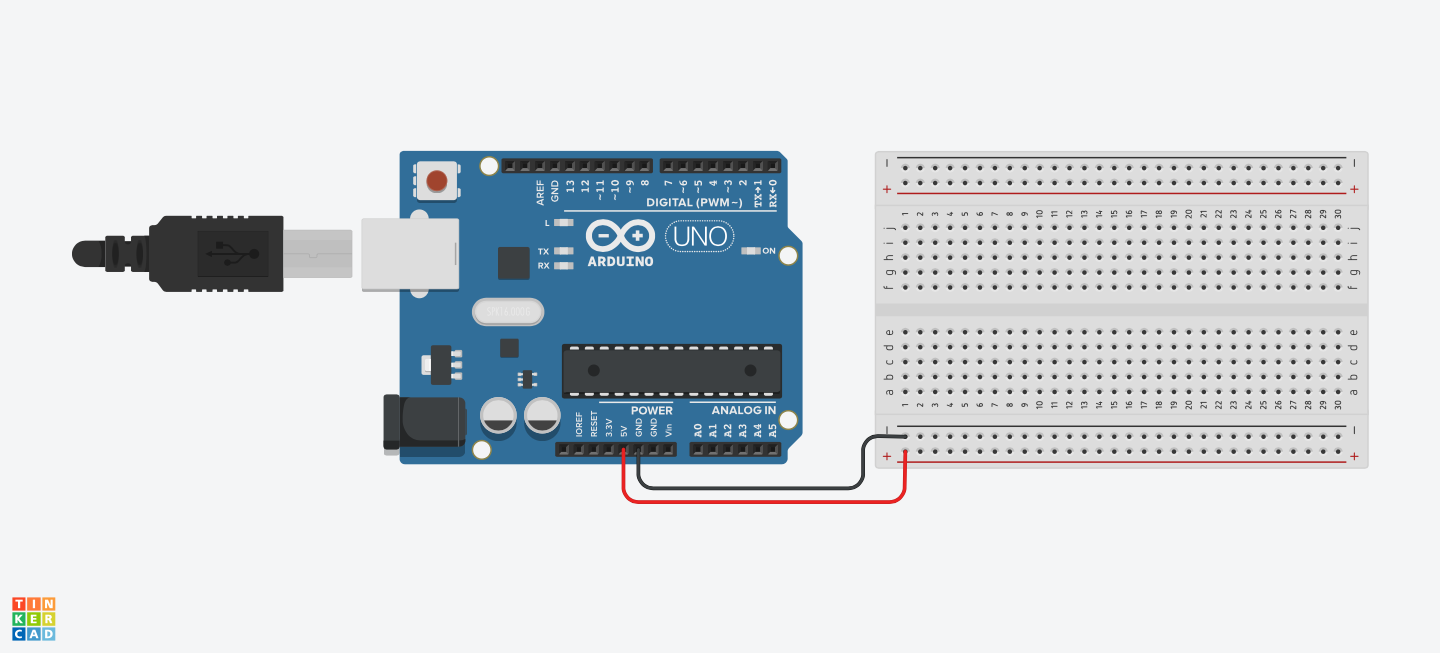
\includegraphics[scale = 0.3]{./Images/circuit1}
		\end{center}
		
		\item Next we want to insert our temperature sensor into the breadboard, be sure to insert it so that all the pins are separated on the breadboard and none of them connect.
		\begin{center}
			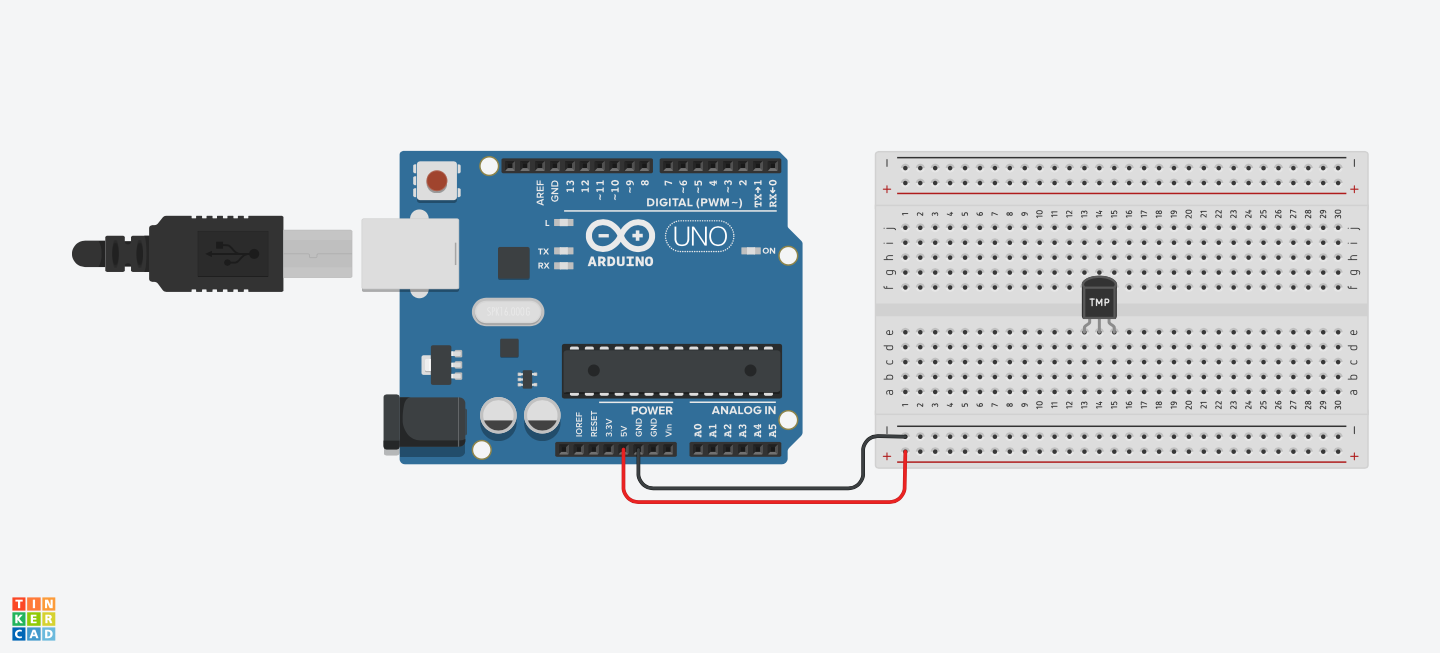
\includegraphics[scale = 0.3]{./Images/circuit2}
		\end{center}
		\item The temp sensor has three pins, one is ground, one is voltage source and one is our output
		\item We need to connect our power to the sensor, connect the Vs to the positive and the GND to the negative sections of the breadboard
		\item Once we have our power connected we need to connect our data pin. From the center data pin we will connect to one of the analog pins on the Arduino. 
		\begin{center}
			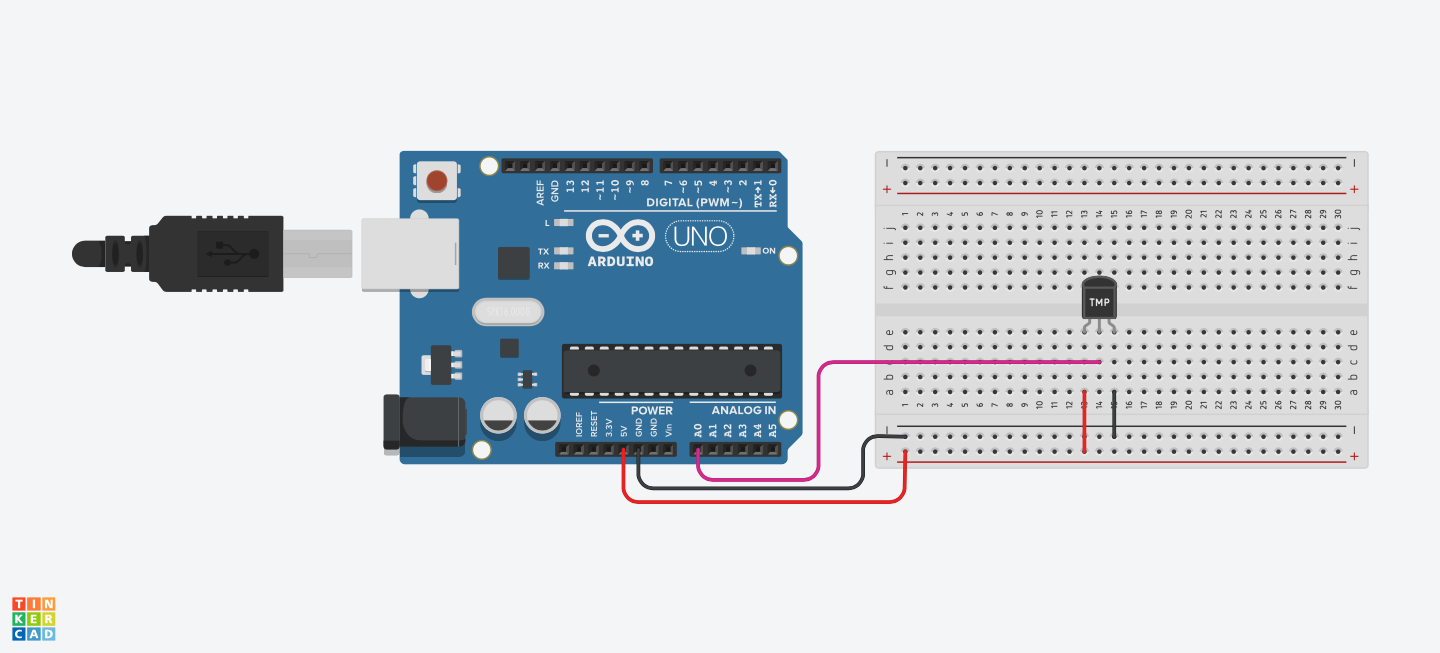
\includegraphics[scale = 0.3]{./Images/circuit3}
		\end{center}
	\end{itemize}
	
	\newpage






 
\section *{Coding For the Sensor}
	\begin{itemize}
		\item We have a way of looking at what our output is.  We will use the serial monitor to print out the values of our analog pins. 
		\item Right now our serial monitor will show a line of text to print out, we want it to print out our analog reading, let's put "read analog pin" into that slot.
		\item To print out the values to serial monitor use the code below:
		\begin{center}
			
\includegraphics[scale = 0.7]{./Images/code1}
		\end{center}
		\item Lets test the code
	\end{itemize}
	
	
	
	
	
	
	
	
	
	
	
	
\section *{Wire The LED}
	\begin{itemize}
		\item We will use an LED to signify to the user when our temperature value has been hit (we will decide this value later). 
		\item Notice that one side of the LED is longer than the other. We will use this to decide which side positive and negative is.
		\begin{itemize}
			\item Anode is positive
			\item Cathode is negative
		\end{itemize}
		\item Put an LED in the breadboard being sure to not cross wires with any other item in the breadboard
		\begin{center}
			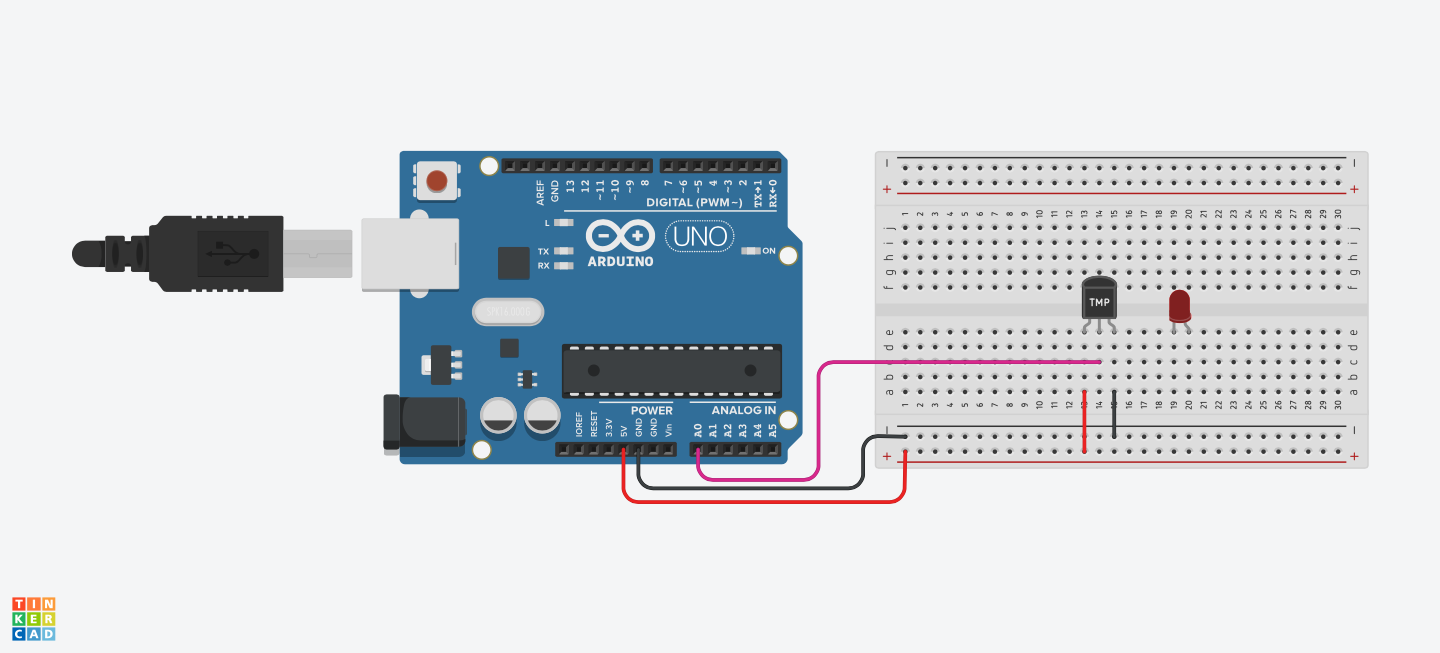
\includegraphics[scale = 0.3]{./Images/circuit4}
		\end{center}
		\item Now an LED cannot be connected without a Resistor.
		\item A resistor limits the amount of energy that can go through the circuit, this keeps the LED from burning up.
		\item Connect a resistor between the cathode side and the negative section of the breadboard.
		\item Lastly we will connect a wire between the Anode of the LED and one of the Digital pins on the Arduino, this will act as our positive lead when we decide we want to turn it on using code.
		\begin{center}
			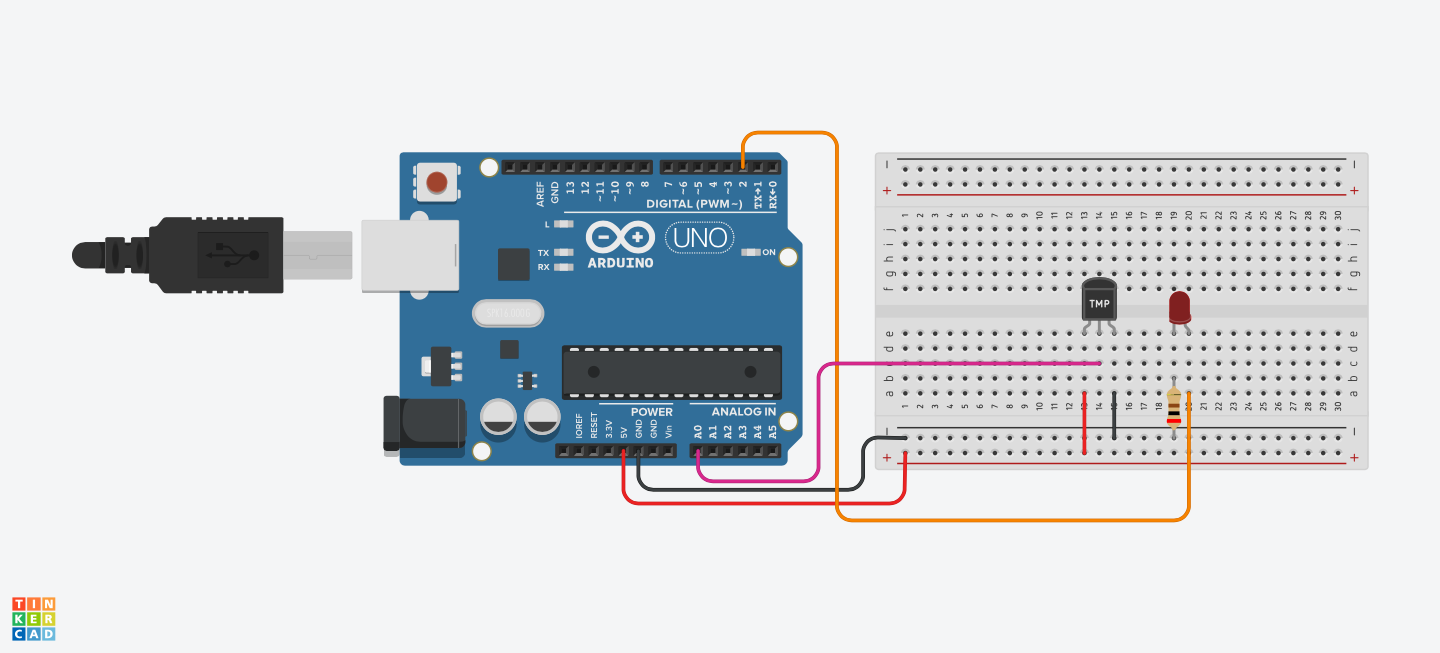
\includegraphics[scale = 0.3]{./Images/circuit5}
		\end{center}
	\end{itemize}
	
	
	
	
	
	
\section *{Code the LED and the Temp Sensor}
	\begin{itemize}
		\item We should build a way for the user to know when we have reached over 104 degrees F.  That is approximately 40 degrees C. 
		\item \textbf{Using the serial monitor what value shows at 40 degrees C?}
		\item We will find the analog value is 184.  
		\item Two things need to happen when looking at these values, above 40 degrees C we will turn and LED on and below it we will turn an LED off.
		\item Let's put in an \textbf{If Then} statement.
		\item We will use a less than operation and compare the \textbf{read analog pin} to the value 184.  This will serve as our boolean check.
		\item If the value is above 184 we will set the LED pin to High
		\newpage
		\item In the else statement, the value of the LED pin will need to be set to LOW in order to turn off the LED
		\item Put the code together to look like this:
		\begin{center}
			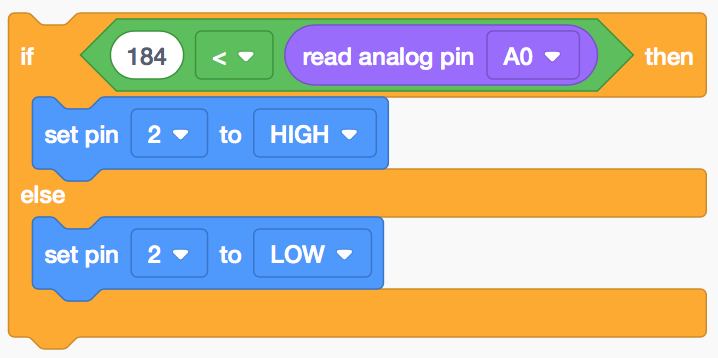
\includegraphics[scale = 0.7]{./Images/code2}
		\end{center}
		\item Now, test it!
	\end{itemize}
	
\end{document}
